\section {Margin maximization classifier}


The hard margin classifier learns the parameters $\mathbf{w} \in \mathbb{R}^n$ and $b \in \mathbb{R}$ of a hyperplane $\mathscr{H} \subset \mathbb{R}^n$, separating two classes of observations $\mathbf{x_i} \in \mathcal{X} \subset \mathbb{R}^n$. To train it, the algorithm takes a set of $m$ observations $\mathbf{x_i}$ together with a vector of labels $y_i = \pm 1$ for each of the observations:

$$
(\mathbf{x_1}, y_1), (\mathbf{x_2}, y_2), \dotsc, (\mathbf{x_m}, y_m)
$$

The learned parameters are then used to define a decision function $f$, assigning to points of $\mathcal{X}$ a label $\pm 1$ corresponding to the side of the hyperplane on which the points stands:

\begin{equation}
  f(\mathbf{x}) = sgn(\langle\mathbf{w}, \mathbf{x}\rangle + b)
\end{equation}

\subsection {Maximizating the margin}

One particularity about the learning algorithm used for Support Vector Machines is the loss function the algorithm tries to optimize. Other learning algorithms typically chose a loss function based on the empirical risk, defined as following for a function $f$ and a training set $(\mathbf{x}, \mathbf{y})$ of size $m$:

\begin{equation}
  R_{\text{emp}}[f] = \frac{1}{m}\sum^m_{i=1}\frac{1}{2}|f(\mathbf{x_i}) - y_i|
\end{equation}

The margin maximization algorithm instead, searches within the space of hyperplanes properly classifying the training set, for the hyperplane with the largest distance from the training points to the hyperplane.

The choice of maximizing the margin has good theoretical roots. Indeed, it is possible to derive an upper bound on the expected missclassification rate of a linear classifier based on the margin of the underlying hyperplane to the training set. It is beyond the scope of this work to go into further details but we will still attempt to provide an intuition on why it might be interesting to optimize it, and for more information the reader can refer to  \textcolor[rgb]{1,0,0}{ref?}.

The intuition comes from the fact that the observations from the test set, or encountered while using the classifier, have been generated by a similar process as the observations present in the training set. Thus, one can assume that observations are very similar to each other up to some noise. Maximizing the hyperplane margin
$M$ is thus the same as increasing the tolerance to noise of the classifier. As shown in figure 1, given a observation $x_i$ from the training set, all new obervations lying in the hypersphere of radius of the margin while be classified similarly to $x_i$.


This idea translates well into the following optimization problem, trying to maximize the margin, while adding a constrain to force the classifier to propery classify the training set

\begin{equation}
  \begin{aligned}
    &\underset{\mathbf{w} \in \mathbb{R}^n, b \in \mathbb{R}} {\text{maximize}}
    & & M := \frac{1}{\|\mathbf{w}\|} \underset{i} {min}\ 
    y_i(\langle\mathbf{w},\mathbf{x_i}\rangle + b)\\
    &\text{subject to}
    & &y_i(\langle\mathbf{w},\mathbf{x_i}\rangle + b) \ge M\ \text{for all}\ i = 1 \dotsc m
  \end{aligned}
\end{equation}

Assuming that a solution to this optimization problem exisits, it still has the issue that although the solution hyperplane is unique, there is an inifity of parameter vectors $\|\mathbf{w}\|$ resulting in the solution hyperplane, only differing in their length. Uniqueness of $\mathbf{w}$ can be ensured by adding to its length the following constraint:

$$M\|\mathbf{w}\| = 1$$

We can thus reformulate the optimization problem into the following quadratic optimization problem which is known to have a numerical solution:

\begin{equation}
  \begin{aligned}
    &\underset{\mathbf{w} \in \mathbb{R}^n, b \in \mathbb{R}} {\text{minimize}}
    & &\|\mathbf{w}\|\\
    &\text{subject to}
    & &y_i(\langle\mathbf{w},\mathbf{x_i}\rangle + b) \ge 1\ \text{for all}\ i = 1 \dotsc m
  \end{aligned}
\end{equation}


\begin{figure*}
  \begin{minipage}{.5\textwidth}
    \centering
    %%% Local Variables:
%%% mode: latex
%%% TeX-master: "learning_with_kernels"
%%% End:


\tikzset{
  noise_pt/.style={solidity,fill=black,draw},  
  pos_pt/.style={circle,minimum width=.4ex, fill=none,draw},
  neg_pt/.style={circle,minimum width=.4ex, fill=black,thick,draw},
  pos_sv/.style={solid,circle,minimum width=.6ex, fill=black,thick,draw=white},
  neg_sv/.style={solid,circle,minimum width=.6ex, fill=none,thick,draw},
}
  
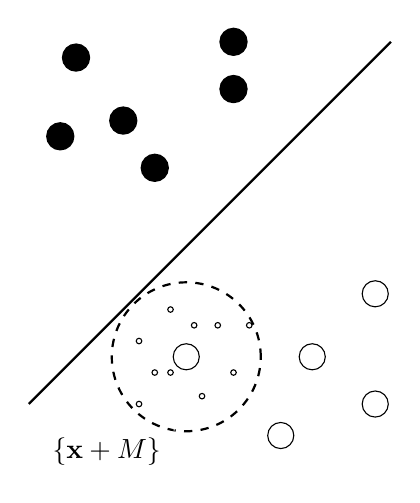
\begin{tikzpicture}[
  scale=2,
  every node/.style={color=black},
  important line/.style={thick},
  dashed line/.style={dashed, thin},
  ]

  \draw[important line]
       (.7,.7) coordinate (lines) -- (3,3) coordinate (linee);

   \foreach \Point in {(1.5,2.2), (.9,2.4), (1.3,2.5), (2,3), (1,2.9), (2,2.7)}{
     \draw \Point node[neg_pt]{};
   }

   \foreach \Point in {(1.7, 1), (2.9,1.4), (2.3,.5), (2.9,.7), (2.5,1)}{
     \draw \Point node[pos_pt]{};
   }

   \draw node[circle,minimum width=12.5ex,fill=none,thick,draw,dashed] at (1.7, 1) {};

   \foreach \Point in {(1.4,1.1),(1.6,.9),(2.0,.9),(1.4,0.7),(1.8,0.75),(1.9,1.2),(2.1,1.2),(1.75,1.2),(1.5, 0.9),(1.6,1.3)} {
     \draw \Point circle[radius=.5pt];
   }

   \draw[dashed, thin,white] (1.7, 1) -- (1.6,0.4)
   node[above, left] {$\{ \mathbf{x} + M \}$};
   
 \end{tikzpicture}

  \end{minipage}%
  \begin{minipage}{.5\textwidth}
    \centering
    %%% Local Variables:
%%% mode: latex
%%% TeX-master: "learning_with_kernels"
%%% End:

\tikzset{
  noise_pt/.style={solidity,fill=black,draw},  
  pos_pt/.style={circle,minimum width=.4ex, fill=none,draw},
  neg_pt/.style={circle,minimum width=.4ex, fill=black,thick,draw},
  pos_sv/.style={solid,circle,minimum width=.6ex, fill=black,thick,draw=white},
  neg_sv/.style={solid,circle,minimum width=.6ex, fill=none,thick,draw},
}
  
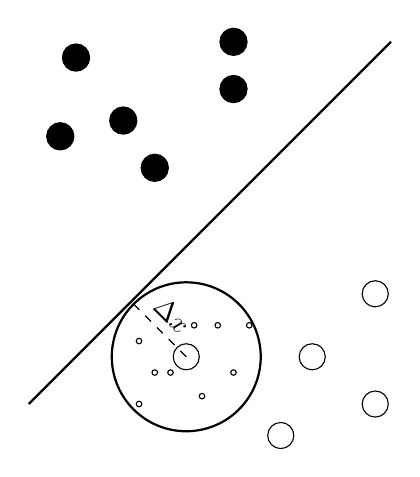
\begin{tikzpicture}[
  scale=2,
  every node/.style={color=black},
  important line/.style={thick},
  dashed line/.style={dashed, thin},
  ]

  \draw[important line]
       (.7,.7) coordinate (lines) -- (3,3) coordinate (linee);

   \foreach \Point in {(1.5,2.2), (.9,2.4), (1.3,2.5), (2,3), (1,2.9), (2,2.7)}{
     \draw \Point node[neg_pt]{};
   }

   \foreach \Point in {(1.7, 1), (2.9,1.4), (2.3,.5), (2.9,.7), (2.5,1)}{
     \draw \Point node[pos_pt]{};
   }

   \draw node[circle,minimum width=12.5ex,fill=none,thick,draw] at (1.7, 1) {};

   \foreach \Point in {(1.4,1.1),(1.6,.9),(2.0,.9),(1.4,0.7),(1.8,0.75),(1.9,1.2),(2.1,1.2),(1.75,1.2),(1.5, 0.9)} {
     \draw \Point circle[radius=.5pt];
   }

   \draw[dashed, thin] (1.7, 1) -- (1.35,1.35)
   node[sloped, above, midway] {$\Delta x$};
   
 \end{tikzpicture}

  \end{minipage}

  \caption{
    Left side illustrates the idea behind margin maximization. Smaller points in the $\{ x + M \}$ are generated by adding noise to an observation of the training set. The right figure shows a dataset separated by a hyperplane with parameters $w, b$. The norm of $w$ is determined by the distance from the plane to the support vectors.
  }
\end{figure*}

\subsection {Support vectors}

Although the previous formulation of the problem helped us to better understand the ideas of support vector machines, the resulting quadratic problem will become impractical when later introducing kernels methods. We will introduce in this section an equivalent formulation of the optimization problem (4) that will not only solve computational issues, but will also give us more insights about the resulting solution.

In order to get to these benefits, we introduce the Lagrangian $L$ together with Lagrange multipliers $\alpha_i \ge 0$:

\begin{equation}
  L(\mathbf{w}, b, \boldsymbol{\alpha}) = \frac{1}{2}\|\mathbf{w}\|^2 - \sum^m_{i=1} \alpha_i[y_i(\langle \mathbf{w}, \mathbf{x_i}\rangle + b)) - 1]
\end{equation}

This is called the dual formulation of our original optimization problem, called the primal problem, in which $\mathbf{w}$ and $b$ are called primal variables, and $\boldsymbol{\alpha}$ the dual variable. It can be shown \textcolor[rgb]{1,0,0}{ref?} that the promal optimization problem is equivalent to finding a saddle point of $L$, minimizing with respect to $\mathbf{w}$ and $b$, while maximizing it with respect to $
\boldsymbol{\alpha}$.

Because the solution of this dual problem is a saddle point, thus an extremum with respect to all variables. Thus our initial constrains are equivalent to the following constrains

\begin{equation}
  \frac{\partial}{\partial b}L(\mathbf{w}, b, \boldsymbol{\alpha}) = 0
  \ \text{and}\ 
  \frac{\partial}{\partial \mathbf{w}}L(\mathbf{w}, b, \boldsymbol{\alpha}) = 0
\end{equation}

leading to

\begin{equation}
  \sum^m_{i=1} \boldsymbol{\alpha}_iy_i = 0
  \ \text{and}\ 
  \mathbf{w} = \sum^m_{i=1} \alpha_iy_i\mathbf{x_i}
\end{equation}

Further, by replacing $(7)$ and $(8)$ in the objective function $(6)$, we obtain an optimization problem free of primal variables, and end up only obtimizing against the vector $\boldsymbol{\alpha}$

\begin{equation}
  \begin{aligned}
    &\underset{\boldsymbol{\alpha} \in \mathbb{R}^n} {\text{maximize}}
    & & W(\boldsymbol{\alpha}) = \sum_{i=1}^m\boldsymbol{\alpha}_i - \frac{1}{2}\sum_{i,j=1}^m\boldsymbol{\alpha}_i\boldsymbol{\alpha}_jy_iy_j\langle\mathbf{x}_i, \mathbf{x}_j\rangle\\
    &\text{subject to}
    & &\boldsymbol{\alpha} \ge 0\ \text{for all}\ i = 1 \dotsc m\\
    & & &\sum^m_{i=1} \boldsymbol{\alpha}_iy_i = 0
  \end{aligned}
\end{equation}

Finally, the Karush-Kuhn-Tucker theorem states that the solution $\boldsymbol{\alpha}$ satisfies the following equality for all $i = 1\dotsc m$
\textcolor[rgb]{1,0,0}{ref?}

\begin{equation}
  \boldsymbol{\alpha}_i[y_i(\langle \mathbf{w}, \mathbf{x_i}\rangle + b) - 1] = 0
\end{equation}

The importance of this equality is twofold. First, it allows us to compute $b$ from an observation $i$ for whichs $\boldsymbol{\alpha}_i \neq 0$. Second and most importantly, this equality implies that every observations not lying on the margin must have a vanishing Lagrangian coefficient. These special observations are called \textit{support vectors}.

Support vectors have a special role. Indeed, looking at (7), one notices that the hyperplane only is only dependent on the support vectors. All other observations vanish from the sum because of their null Lagrange coefficient. This means that all the information extracted from the training set was represented by the support vectors, and all other observations had no role in the training of the algorithm, thus have no role in defining the decision boundary between the two classes of observations.

\subsection{Towards SVMs}

We have chose in this work to present a simplified version of support vector machines called the hard margin classifier. This was done in order to focus on building an intuition of the way support vectors machines work. In practice, several considerations have to be made in order to make this classifier usable. These points will be handled in the next paragraphs.

The most important addition to the margin maximization algorithm that we have omited so far is the ability to train on a non linearly separable dataset caused by noise is the observations. Indeed, real world datasets are often generated from measuring physical phenomena. This kind of dataset is subject to noise that can cause an overlapping of the two classes around the decision boundary. Thankfully, these issues can be mitigated by introducing slack variables that will compensate the offset of an observation in the direction of the other class. Figure X illustrate the concept of these slack variables. A thorough investigation of this method can be found in  \textcolor[rgb]{1,0,0}{ref?}.

%%% Local Variables:
%%% mode: latex
%%% TeX-master: "learning_with_kernels"
%%% End:
